\documentclass[tikz]{standalone}

\usepackage{graphicx}
\usepackage{tikz}
\usetikzlibrary{arrows.meta, automata, positioning, quotes}

\tikzstyle{every picture} = [node distance=1.3cm]


\begin{document} 
        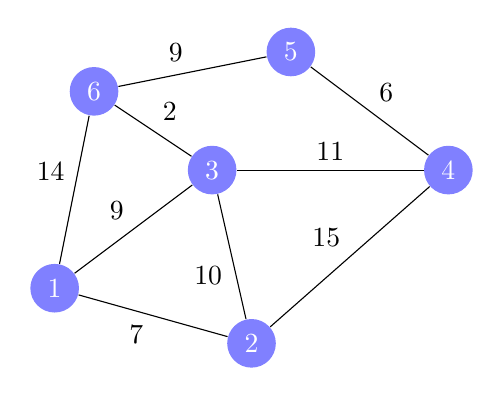
\begin{tikzpicture} 
            \node (node 1) at(0,1) [circle,double, double distance =1.2pt,text=white,fill=blue!50,] {1};
            \node (node 2) at(2.5,0.3) [circle,double, double distance =1.2pt,text=white,fill=blue!50,] {2};
            \node (node 3) at(2,2.5) [circle,double, double distance =1.2pt,text=white,fill=blue!50,] {3};
            \node (node 4) at(5,2.5) [circle,double, double distance =1.2pt,text=white,fill=blue!50,] {4};
            \node (node 5) at(3,4) [circle,double, double distance =1.2pt,text=white,fill=blue!50,] {5};
            \node (node 6) at(0.5,3.5) [circle,double, double distance =1.2pt,text=white,fill=blue!50,] {6};
            
            
            \path 	(node 2) edge[-,"7"] (node 1)
            		(node 1) edge[-,"14"] (node 6)
            		(node 1) edge[-,"9"] (node 3)
            		(node 2) edge[-,"15"] (node 4)
            		(node 2) edge[-,"10"] (node 3)
            		(node 6) edge[-,"2"] (node 3)
            		(node 3) edge[-,"11"] (node 4)
            		(node 5) edge[-,"6"] (node 4)
            		(node 6) edge[-,"9"] (node 5);
            		
            
                  

        \end{tikzpicture}
\end{document}